\chapter{Formatting Guide}
\label{chap:formatting_guide}

\section{Margins}

This template follows the UNC graduate school thesis/dissertation formatting guide as rigidly as possible.
This template has uniform margins throughout the entire document:
\begin{itemize}
    \item Left: 1''
    \item Right: 1''
    \item Top: 1''
    \item Bottom: 1''
\end{itemize}

\section{Font}
A TrueType font is recommended/required by the ProQuest dissertation publishing. Recommended fonts and sizes can be found in \autoref{tab:font}.

\begin{table}
    \centering
    \caption{Recommended font type and size}\label{tab:font}
    \begin{tabular}{ll}
        \toprule
        Font name            & Font Size \\ \midrule
        Arial                & 10pt\\
        Century              & 11pt\\
        Courier New          & 10pt\\
        Garamond             & 12pt\\
        Georgia              & 11pt\\
        Lucida Bright        & 10pt\\
        Microsoft Sans Serif & 10pt\\
        Tahoma               & 10pt\\
        Times New Roman      & 12pt\\
        Trebuchet MS         & 10pt\\
        Verdana              & 10pt\\ \bottomrule
    \end{tabular}
\end{table}

If you're using \texttt{pdflatex} to compile this template, include the \texttt{times} package in the preamble.
If you're using \texttt{xelatex} to compile this template, you can use the \texttt{fontspec} package and the \texttt{setmainfont} command to choose your favorite font.
This template by default uses 12pt Times New Roman.

\section{Spacing and Indentation}

The template takes care of spacing and indentation:
\begin{itemize}
    \item Text appears in a single column on each page and is double-spaced throughout the document.
    \item New paragraphs are indicated by a consistent tab indentation throughout the entire document.
    \item The document text is left-justified.
    \item For blocked quotations, indent the entire text of the quotation consistently from the left margin.
\end{itemize}

\lipsum[6]
\begin{quote}
    This is an example showing the indentation of block quoted text.
    \lipsum[8]
\end{quote}
\lipsum[7]

\section{Pagination}
This template takes care of pagination.

Pagination and margin are also well maintained for landscape pages.
\begin{landscape}
    \lipsum[9] Let's also see how does footnote works in landscape pages~\footnote{We have a footnote in landscape environment}.
\end{landscape}

\section{Footnotes and Endnotes}
Footnotes\footnote{\lipsum[10]} and endnotes\footnote{\lipsum[11]} obey the
formatting guide. However, using both of them confuses the note numbering.
Given the discrepancy between the official format guide\endnote{\lipsum[12]}
and the official sample pages\endnote{\lipsum[14]}, the correct order for
endnotes and appendixes are unclear.  Thus, using only footnote is recommended.

\section{Tables and Figures}
Tables, figures, and illustrations vary widely by discipline. Therefore, formatting of these
components is largely at the discretion of the author.

List of figures and list of tables are well taken care of by \LaTeX{} and this
template.  If an entry in LOT/LOF takes up more than one line, break up the
entry about three-fourths of the way across the page and place the rest of the
text on a second line, single-spacing the two lines.

One nice trick is the short caption option for the
\texttt{\textbackslash{}caption{}} command.  It allows the LOT/LOF only include
the short caption but not the full caption.
\begin{figure}
    \centering
    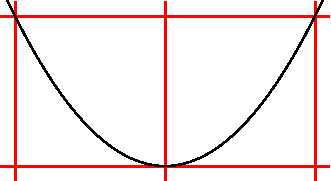
\includegraphics[width=0.5\textwidth]{figures/demo.pdf}
    \caption{A very long caption that does not make much sense but only tests the line-breaking and line-spacing in LOT/LOF.}
\end{figure}

\begin{figure}
    \centering
    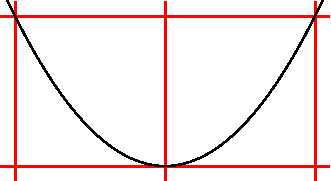
\includegraphics[width=0.5\textwidth]{figures/demo.pdf}
    \caption[Short Caption]{A very long caption that does not make much sense but only tests the line-breaking and line-spacing in LOT/LOF.}
\end{figure}

\section{Reference}
The APA style is used for references. Notice the differences caused by different citation command.

\begin{table}
    \centering
    \caption[Short title]{Comparison of different citation command.}\label{tab:citation}
    \begin{tabular}{ll}
        \toprule
Command                        & Results \\ \midrule
\texttt{\textbackslash{}cite}  & \cite{LFR}\\
\texttt{\textbackslash{}citep} & \citep{LFR}\\
\texttt{\textbackslash{}citet} & \citet{LFR}\\\bottomrule
    \end{tabular}
\end{table}

\section{Length}
There are no requirements for the length of the PhD thesis. For the Department of Computer Science, from 2014 to 2017, average length of the thesis main body text is $\mu \approx 120, \sigma \approx 33$, average length of main body text + reference is $\mu \approx 129, \sigma \approx 35$.